%!TEX root = main.tex

\subsection{\textbf{RQ1:} What processes do software developers utilize for merge conflicts?}\label{RQ1}

\begin{figure}[!htbp]
\centering
\fbox{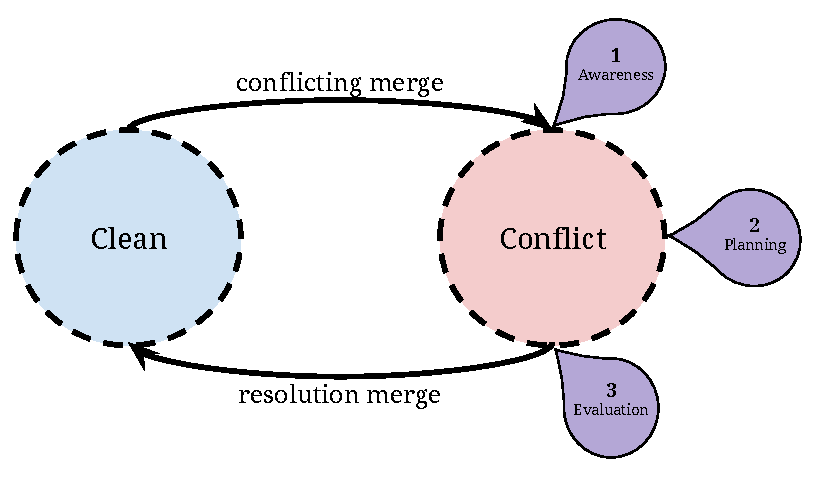
\includegraphics[width=0.98\textwidth,keepaspectratio]{imgs/MergeConflictModel}}
\caption{Model of Developer Processes for Merge Conflicts. Developers alternate between \textit{clean} and \textit{conflicting} states within their codebase. Developers maintain \textit{awareness}~(1) of conflicts within the codebase in different ways. Once aware, developers \textit{plan}~(2) a solution to fix the conflict. And finally, developers \textit{evaluate}~(3) the effectiveness of their deployed resolutions.}
\label{model}
\end{figure}

\boldif{Results from interviews indicated that a common model of operating with merge conflicts exists.}

\boldif{\textit{Add anecdotal quotes and descriptions from interviews to highlight these observations.}}

\boldif{Based on these anecdotal observations, we construct an initial model of the processes that developers employ when working with merge conflicts, see Fig.~\ref{model}.}
 
\boldif{To explore and validate this model, we asked developers to reflect upon how they become aware of merge conflicts, how they plan for merge conflict resolutions, and how they evaluate their merge conflict resolutions in the \textit{Processes Survey}~(S1).}
 
\boldif{We present the results to these research questions in Section~\ref{RQ1a}, \ref{RQ1b}, and \ref{RQ1c}.}

\subsection{\textbf{RQ1a:} How do software developers become aware of merge conflicts?}\label{RQ1a}

\begin{table}[!htbp]
\renewcommand{\arraystretch}{1.3}
\caption{Merge Awareness Toolsets (Top 10) from Processes Survey (S1)}
\label{s1_toolset}
\centering
\begin{tabularx}{\textwidth}{c|rl}
\toprule
  \parnoteclear % tabularx will otherwise add each note thrice
  \# Participants (\%)\parnote{Survey participants were allowed to provide multiple tools. Each entry represents the number of participants that responded with that particular tool, along with the percentage of the overall tool responses (126 responses). 57 out of 102 respondents (56\%) indicated the use of at least one merge awareness tool.} & Tool & Description\\
\midrule
  32 (25.40\%) & Git & Version Control System\\
  7 (5.56\%) & Email (unspecified) & Email Client or System\\
  7 (5.56\%) & GitHub & Website\\
  4 (3.17\%) & SVN & Version Control System\\
  4 (3.17\%) & Visual Studio & IDE\\
  3 (2.38\%) & PagerDuty & IT Incident Response Platform\\
  3 (2.38\%) & GitLab & Website\\
  3 (2.38\%) & Jenkins & Continuous Integration Platform\\
  3 (2.38\%) & Team Foundation Server & Version Control System\\
  3 (2.38\%) & VCS (unspecified) & Version Control System\\
\bottomrule
\end{tabularx}
\parnotes
\end{table}

To understand the processes that software developers employ to maintain awareness of the state of code, we asked Processes Survey (S1) participants to categorize and describe their monitoring processes: whether and how they monitor for merge conflicts, and how they determine the urgency of any merge conflicts that occur.

We found that 32.26\% of participants do not monitor for merge conflicts during their development sessions.
For the 67.74\% participants that indicate \textit{yes} or \textit{sometimes} to the question of monitoring for merge conflicts, we asked them to describe the processes and tools that they use for monitoring.

We identified 61 different tools from the 126 responses.
Some mentioned generic responses such as \textit{``email''}, for which we create a separate category.
Table~\ref{s1_toolset} lists the top 10 most common tools used by participants to monitor for merge conflicts.

In examining the list of these tools, we note that developers most often use version control systems (e.g. Git, SVN, TFS, and unspecified VCS) to handle tracking changes, and potentially identifying merge conflicts, within a codebase.
In this list, there is also one continuous integration (CI) platform (Jenkins), an IT incident response platform (PagerDuty), and two VCS-hosting websites (GitHub and GitLab).
This indicates that developers are currently relying on reactive tools that indicate the presence of merge conflicts after they have been introduced to a codebase.

We then evaluated responses based on whether described processes were proactive or reactive in nature (using card sorting and negotiated agreement).
We find that 42 of 57 responses (73.68\%) described reactive processes for monitoring for merge conflicts.
Combined with the tools used, we find that developers are currently not leveraging the functionalities provided by many research prototypes (e.g., Palantir~\cite{palantir}, Crystal~\cite{Brun2011}) that are specifically designed to facilitate proactive conflict detection.

In addition, we identified \textbf{X} distinct categories of processes that developers use to monitor for merge conflicts (see Table~\ref{s1_monitoring_processes}).
 \textit{Provide further discussion on the results; analysis between Caius and Nick still needed to group the processes in groups}

\subsection{\textbf{RQ1b:} How do software developers plan for merge conflict resolutions?}\label{RQ1b}

\subsection{\textbf{RQ1c:} How do software developers evaluate merge conflict resolutions?}\label{RQ1c}